%%% License: Creative Commons Attribution Share Alike 4.0 (see https://creativecommons.org/licenses/by-sa/4.0/)
%%% Slides are based heavily on earlier versions of this course taught by Jesper Rudiger.

\documentclass[english,10pt
%,handout
,aspectratio=169
]{beamer}
%%% License: Creative Commons Attribution Share Alike 4.0 (see https://creativecommons.org/licenses/by-sa/4.0/)
%%% Slides are based heavily on earlier versions of this course taught by Jesper Rudiger and Peter Norman Sorensen.

\DeclareGraphicsExtensions{.eps, .pdf,.png,.jpg,.mps,}
\usetheme{reMedian}
\usepackage{parskip}
\makeatother

\renewcommand{\baselinestretch}{1.1} 

\usepackage{amsmath, amssymb, amsfonts, amsthm}
\usepackage{enumerate}
\usepackage{hyperref}
\usepackage{url}
\usepackage{bbm}
\usepackage{color}

\usepackage{tikz}
\usepackage{tikzscale}
\newcommand*\circled[1]{\tikz[baseline=(char.base)]{
		\node[shape=circle,draw, inner sep=-20pt] (char) {#1};}}
\usetikzlibrary{automata,positioning}
\usetikzlibrary{decorations.pathreplacing}
\usepackage{pgfplots}
\usepgfplotslibrary{fillbetween}
\usepackage{graphicx}

\usepackage{setspace}
%\thinmuskip=1mu
%\medmuskip=1mu 
%\thickmuskip=1mu 


\usecolortheme{default}
\usepackage{verbatim}
\usepackage[normalem]{ulem}

\usepackage{apptools}
\AtAppendix{
	\setbeamertemplate{frame numbering}[none]
}
\usepackage{natbib}



\title{Financial Markets Microstructure \\ Lecture 4}

\subtitle{Informative Order Flow\\
	Chapter 3.1-3.3 of FPR}

\author{Egor Starkov}

\date{K{\o}benhavns Unversitet \\
	Spring 2022}



\begin{document}
\AtBeginSection[]{
	\frame<beamer>{
		\frametitle{This lecture:}
		\tableofcontents[currentsection,currentsubsection]
}}
\frame[plain]{\titlepage}

%\section{Revision}

\begin{frame}{What did we do last week?}
\begin{enumerate}
	\item Discuss liquidity
	\item Talk about different measures of:
	\begin{itemize}
		\item spreads (quoted, effective, realized)
		\item depth and price impact
		\item execution costs
	\end{itemize}
	\item Estimators for missing data
	\begin{itemize}
		\item Lee-Ready algorithm for estimating trade direction
		\item Roll's spread estimator requiring only price data
	\end{itemize}
\end{enumerate}
\end{frame}


%\begin{frame}{Exercises from last week}
%	\begin{itemize}
%		%\item In Absalon, I have attached a commission and fee schedule from Robinhood Financial. More information on \url{www.robinhood.io/}. Discuss the potential effect on other brokerage services.
%		\item In this course we mostly imply equity markets. Read the article (on Absalon) about corporate bond markets. Discuss how differences in market structures of stock and bond markets affect liquidity in these markets.
%		\item \textcolor{gray}{Recreate the graphs and figures and numbers I presented [last week] using the KrispyKreme dataset}
%		\item \textcolor{gray}{Solve exercise 8 regarding implementation shortfall, on page 75 in the textbook.
%		Discuss the meaning of $m_t$ in this analysis.}
%	\end{itemize}
%\end{frame}


\begin{frame}{Overview}
	Before we start, let's look at an overview of what we'll do in the rest of the course
	
	\textbf{Part 1}: Setting up the models
	\begin{itemize}
	\item Dealer models 1; \structure{Glosten-Milgrom}, fixed trade size; Bayes' Rule; adverse selection
	\item Dealer models 2; \structure{Kyle}, variable trade size; market depth; estimating liquidity determinants, inventory risk
	\item Limit order book; \structure{Glosten}: static, random market order demand; market design; \structure{Parlour}: dynamic, endogenous market order demand
	\end{itemize}
\end{frame}


\begin{frame}{Overview}
\textbf{Part 2}: Applying the models
\begin{itemize}
	\item Fragmentation: costs and benefits
	\item Transparency: search costs and order flow transparency
	\item Value of liquidity
	\item Liquidity and corporate policy
\end{itemize}
\end{frame}


\begin{frame}{Overview}
\textbf{Part 3}: Topics and specialized models
\begin{itemize}
	\item High-frequency trading (\structure{Biais et al.}, \structure{Budish et al.})
	\item Public information; optimal disclosure policies; public announcements and trade volumes (\structure{Kondor})
	\item Bubbles; herding; common knowledge (\structure{Smith and S{\o}rensen}, \structure{Abreu and Brunnermeier})
	\item Auctions (bonus class)
\end{itemize}
\end{frame}


\begin{frame}{Today}
\begin{enumerate}
	\item Beginning of a long discussion about determinants of the spread
	\item Go in-depth with the relation between information and prices
	\item What is informational efficiency?
	\item Discuss Glosten and Milgrom's model of information-based trading
	%\item Analyze through the model what drives the spread 
\end{enumerate}
\end{frame}



\section{Information and Prices}

\begin{frame}{Determinants of liquidity}
	\begin{itemize}[<+->]
		\item Last week: \alert{illiquidity} $\Rightarrow$ deviation of realized prices from the asset's fundamental value.
		\item Source of illiquidity: \visible<handout:0>{\alert{market thinness}}. Or so I told you...
		\item If that was the only reason, trivial solution for efficiency: \visible<handout:0>{add many dealers}.
		\begin{itemize}
			\item Unsurprisingly, this does not close the spread.
		\end{itemize}
		\item So \structure{what drives the spread}?
		\begin{itemize}
			\item To answer that, first talk about \structure{what drives the prices}.
		\end{itemize}
	\end{itemize}
\end{frame}


\begin{frame}{Price determinants}
	Stock prices move around all the time
	\begin{itemize}
		\item Media reports are full of ex post rationalizations 
		%\item Look at CNN Money reports (on absalon)
		\item But these can be pretty arbitrary (see \href{https://www.smbc-comics.com/comic/markets}{\uline{this SMBC comic}} and \href{https://twitter.com/stonksgoingUP1}{@stonksgoingUP1} on twitter)
	\end{itemize}
	What actually determines stock prices and their movement?
\end{frame}


\begin{frame}{Price determinants}
	In this course: everybody agrees on assets' future cash flows ($\approx$value), \textit{conditional} on fundamentals. Broadly speaking, three reasons for trading:
	\begin{itemize}
		\item \textbf{Risk}: Getting the right risk profile (relevant to trader)
		\item (Funding) \textbf{Liquidity}: Trader needs liquid funds or has excess funds to invest (relevant to trader)
		\item \textbf{Speculation}: Different expectations of fundamentals because different \alert{information} (relevant to everyone)
	\end{itemize}
\end{frame}


\begin{frame}{Types of information}
	\begin{itemize}
		\item Different types of information (it's a spectrum really)
		\begin{itemize}
			\item \textbf{Public information}:  asset price may move \textit{without} trade
			\item \textbf{Private information} possessed by some traders  $\rightarrow$ reveal this information through their trading
		\end{itemize}
		\pause
		\item Draw a wedge between \alert{legal} and \structure{academic} ($\leftarrow$ \structure{our}) definitions of \textbf{private information}
		\begin{itemize}
			\item \alert{Legal}: insider info is that which is only available to a restricted number of people. Trading based on insider info is illegal in most jurisdictions.
			\item \structure{Academic}: some agents may be better at analyzing publicly available info, thus have better info about fundamentals.
		\end{itemize}
	\end{itemize}
\end{frame}


\begin{frame}<handout:0>{Information and prices}
	\begin{quotation}
		``Fundamentally, in a system in which the knowledge of the relevant facts is dispersed among many people, prices can act to coordinate the separate actions of different people.'' -- \structure{Von Hayek}
	\end{quotation}
	\pause
	
	\structure{Fama}'s \textbf{efficient markets hypothesis}: {prices} must be {efficient}.
	\\
	I.e., they must reflect all available information. Example: next slide
\end{frame}


\begin{frame}{How Dr. Alchian learned to build the bomb}
	\small 
	\begin{quote}
		We knew they were developing this H-bomb, but we wanted to know, what's in it? What's the fissile material? Well there's thorium, thallium, beryllium, and something else, and we asked Herman Kahn and he said, ‘Can't tell you’… I said, ‘I'll find out’, so I went down to the RAND library and had them get for me the US Government's Dept. of Commerce Yearbook which has items on every industry by product, so I went through and looked up thorium, who makes it, looked up beryllium, who makes it, looked them all up, took me about 10 minutes to do it, and got them. There were about five companies, five of these things, and then I called Dean Witter… they had the names of the companies also making these things, ‘Look up for me the price of these companies…’ and here were these four or five stocks going like this, and then about, I think it was September, this was now around October, one of them started to go like that, from \$2 to around \$10, the rest were going like this, so I thought ‘Well, that's interesting’… I wrote it up and distributed it around the social science group the next day. I got a phone call from the head of RAND calling me in, nice guy, knew him well, he said ‘Armen, we've got to suppress this’… I said ‘Yes, sir’, and I took it and put it away, and that was the first event study.
		\begin{flushright}
			--from a 2000 interview with A.Alchian, transcribed by \cite{newhard_stock_2014}
		\end{flushright}
	\end{quote}
\end{frame}


%\begin{frame}{Information and prices}
%	\centering
%	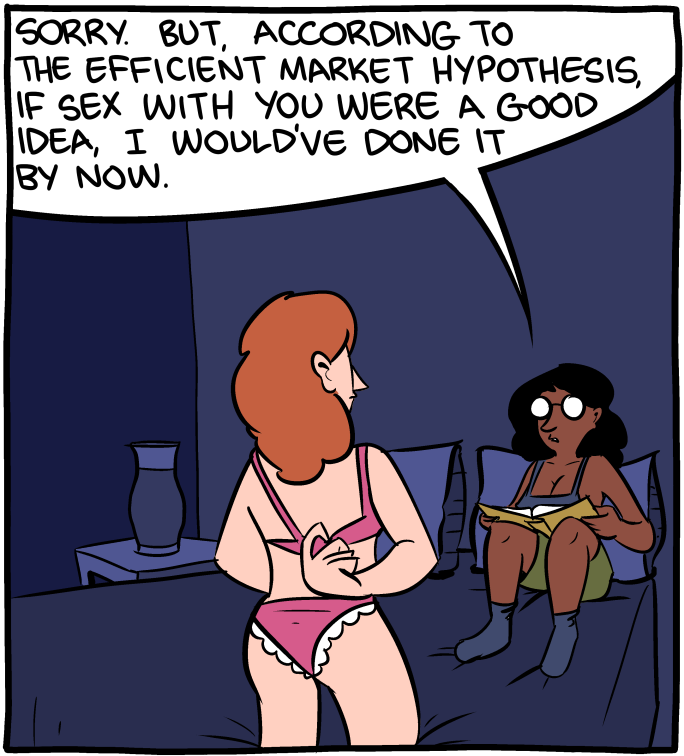
\includegraphics[scale=0.25]{pics/20140603.png}
%	
%	\url{https://smbc-comics.com}
%\end{frame}


\begin{frame}{Types of informational efficiency}
	There are different kinds of price efficiency:
	\begin{itemize}
		\item \textbf{Weak form}: Prices reflect historic (price) information
		\item \textbf{Semi-strong form}: Prices reflect all public information
		\item \textbf{Strong form}: Prices reflect all public and private information
	\end{itemize}
	Strong is the kind of efficiency we had in mind in the previous lectures. It arises in classical models in Economics (see General Equilibrium theory)
\end{frame}


\begin{frame}{Issues with EMH}
Issues with EMH:
\begin{itemize}[<+->]
	\item \textbf{No-trade theorem}: If traders have private information and care only about fundamentals, nobody should ever trade (\cite{milgrom_information_1982})
	\item \textbf{GS informational paradox}: (\cite{grossman_impossibility_1980})
	\begin{itemize}
		\item Suppose markets were informationally efficient, then prices would reflect traders' private information
		\item Thus: no incentive to acquire information (if this is costly)
	\end{itemize} 
	\item \textbf{Volatility}: prices move a lot, such volatility cannot be justified by public news alone
	\item \textbf{Process}: \alert{how} does information get incorporated into prices?
\end{itemize}
\pause[6]
So we will not take EMH for granted, but rather see whether it arises in models endogenously.
\end{frame}


\begin{frame}{Asset value}
	\begin{itemize}
		\item Let's try to figure out how price efficiency looks like in math.
		\item \structure{Information}: $\Omega_t$ captures the market's (public) knowledge at time $t$ -- ever more is known: 
		\structure{$\Omega_{t+1}=(\Omega_t, I_{t+1})$}. 
		
		\item \structure{Market valuation} ($\neq$ price) of an asset = expectation of underlying \structure{fundamental value} $v$ given information $\Omega_{t}$:
		\begin{align*}
			\mu_t &= \mathbb{E} \left[ v | \Omega_t \right].
		\end{align*}
		Think of $v$ as the sum of discounted cash flows: $v = \sum_{s=t}^{\infty} \delta^{s-t} c_s$ (uncertain at $t$).
	\end{itemize}
\end{frame}


\begin{frame}{Informational efficiency (1)}
\begin{itemize}
	\item Informational efficiency then corresponds to: \structure{$p_t = \mu_t = \mathbb{E}[v|\Omega_t]$}
	\\
	($\Omega_t$ is ``market's knowledge'', so efficiency understood as semi-strong)
	\item Valuation only changes if new information arrives: `innovation in value' is a random variable: \structure{$\epsilon_{t+1} = \mu_{t+1} - \mu_t$}. Then
	\begin{align*}
		\mathbb{E}[\epsilon_{t+1}|\Omega_t] 
		& = \mathbb{E}[\mu_{t+1} - \mu_t|\Omega_t]\\
		& = \mathbb{E}[\mu_{t+1}|\Omega_t] - \mathbb{E}[\mu_t|\Omega_t]\\  
		& = \mathbb{E}[ \mathbb{E}[v|\Omega_{t+1}]|\Omega_t] - \mu_t\\  
		& = \mathbb{E}[v|\Omega_t] - \mu_t\\  
		& = \mu_t- \mu_t\\  
		& = 0.
	\end{align*}
\end{itemize}
\end{frame}


\begin{frame}{Informational efficiency (2)}
	\begin{itemize}
	 \item Also, $\mathbb{E}[\epsilon_{s}\epsilon_t]=0$, $\forall s \ne t$.
	\item Price innovation is equal to the valuation innovation:
	\[
	p_{t+1} - p_t = \mu_{t+1} - \mu_t = \epsilon_{t+1}
	\]
	\item Thus
	\[
	\mathbb{E}[p_{t+1}|\Omega_{t}] = p_t
	\]
	\item When we have informational efficiency, the price is a \alert{martingale}
\end{itemize}
\end{frame}



\section{Glosten-Milgrom model}

\begin{frame}{\cite{glosten_bid_1985}}
	\begin{quotation}
		All models are wrong; some models are useful.
		\begin{flushright}
			-- \structure{George Box}
		\end{flushright}
	\end{quotation}
\end{frame}


\begin{frame}{GM85: Overview}
	\begin{itemize}
		\item The simplest model explaining \structure{spread} through private information.
		\item Spread is driven by adverse selection
		\item Dynamic model, periods $t = 1,2,...$
		\item Two players in every period:
		\begin{itemize}
			\item trader and dealer
			\item \alert{dealer} long-lived; trader new every period
			\item \alert{trader} can be informed or not
		\end{itemize}
	\end{itemize}
\end{frame}



\begin{frame}{GM85: Model (1)}
	\textbf{Trader:} is either a speculator or a noise trader, can submit a market order to buy or sell one unit of the asset.
	\begin{itemize}
		\item \structure{Speculator} (probability $\pi$): has private information.
		\begin{itemize}
			\item Risk neutral, chooses his market order $d$ to maximize expected profits:
			\begin{equation*}
				d_t= \left\{
				\begin{aligned}
				1	& \text{ if buy}; \\
				0	& \text{ if abstain}; \\
				-1	& \text{ if sell}.
				\end{aligned}
				\right.
			\end{equation*}
			\item `Hides' behind noise traders
		\end{itemize}
		\item \structure{Noise trader} (probability $1-\pi$): trades for exogenous reasons (hedging, liquidity).
		\begin{itemize}
			\item Buys with fixed probability $\beta_B$; sells w.p. $\beta_S$; abstains w.p. $1-\beta_B - \beta_S$
			\item \alert{Important}: we often assume that these traders behave in a certain way (behavior types) but they can be perfectly rational!
		\end{itemize}
	\end{itemize}
\end{frame}


\begin{frame}{GM85: Model (2)}
	\textbf{Dealer (market maker)}
	\begin{itemize}
		\item Risk neutral
		\item Willing to trade \alert{exactly one unit} (buy/sell/no trade) each period
		\item Sets \alert{bid and ask prices} (for a single unit)
		\item Quote price before seing trade (limit order)
		\item Does not know whether trader is speculator or noise trader
		\item \structure{Competitive}: prices=expected asset value conditional on information
		\item Trading is sequential: market orders served one by one
	\end{itemize}
\end{frame}


\begin{frame}<handout:0>{Aside on Dealers}
	\begin{quotation}
		\small ``For each security in which a member is registered as a Market Maker, the member shall be willing to buy and sell such security for its own account on a continuous basis during regular market hours and shall enter and maintain a two-sided trading interest (``Two-Sided Obligation'') that is identified to the Exchange as the interest meeting the obligation and is displayed in the Exchange's quotation montage at all times.''
		\begin{flushright}
			-- Nasdaq Rule 4613
		\end{flushright}
	\end{quotation}
	\vspace{3ex}
	\begin{quotation}
		\small ``Minimum requirements: at least 85\% of the time, at most 4\% bid-offer
		spread, order size at least worth 4,000 euros''
		\begin{flushright}
			-- Nasdaq OMX Helsinki
		\end{flushright}
	\end{quotation}
\end{frame}


\begin{frame}{GM85: Model (3)}
\begin{itemize}
	\item \textbf{Asset value}:
	\begin{itemize}
		\item Random asset value $v$ drawn from distribution
		\item Assume $v$ is the fundamental (terminal) value
		\item Speculators know $v$ perfectly (not much changes if they don't)
	\end{itemize}
	\item \textbf{Equilibrium}:
	\begin{itemize}
		\item An equilibrium consists of \structure{bid and ask prices} and \structure{speculator's strategy}
		\item They must be such that: (i) prices are competitive (zero profit for MM), (ii) speculator best-responds to prices (maximizes expected gain).
	\end{itemize}
\end{itemize}
\end{frame}


\begin{frame}{Some questions}
\begin{itemize}[<+->]
	\item Why are there no uninformed speculators?
	\item What is the role of the dealer? What functions does he fulfill?
	\item Why is the dealer willing to trade with better-informed speculators?
\end{itemize}
\end{frame}


\begin{frame}{Analysis. A: Market making}
\begin{itemize}[<+->]
	\item Dealer quotes bid and ask prices on \textit{one unit}
	\begin{itemize}
		\item Can revise prices between each incoming trade
	\end{itemize}
	\item Quoted ask price $a_t$ only relevant if next incoming trader decides to buy
	\begin{itemize}
		\item Same for bid $b_t$
	\end{itemize}
	\item Risk neutrality and competition implies that the \structure{ask price} and \structure{bid price} are
	\begin{align*}
		a_t & = \mathbb{E}[v|\Omega_{t-1}, Buy]; \\
		b_t &= \mathbb{E}[v|\Omega_{t-1},  Sell].
	\end{align*}
	\item Notice that both sides of the equality depend on prices
\end{itemize}
\end{frame}


\begin{frame}{Analysis. B: Informed trading}
\begin{itemize}
	\item Speculator knows $v$. Given prices $a_t$ and $b_t$, the expected profits $\Pi$ are:
	\begin{equation*}
		\Pi(v,a_t,b_t,d_t)= \left\{
		\begin{aligned}
		&v - a_t  	&& \text{ if } d_t=1; \quad && (Buy)\\
		&0			&&\text{ if } d_t=0; \quad && (Abstain)\\
		&b_t - v 	&& \text{ if } d_t=-1. \quad && (Sell)
		\end{aligned}
		\right.
	\end{equation*}
	\pause
	\item Speculator's best response to $(a_t,b_t)$ is: (assume $a_t \geq b_t$)
	\begin{itemize}
		\item Buy when $v > a_t$, i.e. when $v$ is large enough
		\item Sell when $v<b_t$, i.e. when $v$ is small enough
		\item Abstain if $a_t > v > b_t$
	\end{itemize}
\end{itemize}
\end{frame}


\begin{frame}{Analysis. C: Equilibrium definition}
Dealer must make zero profit ({competition}), traders must trade optimally.
This gives us two \structure{equilibrium conditions}.
\begin{itemize}
	\item Let $\sigma_t$ denote the speculator's strategy, where $\sigma_t(d_t|v)$ is the probability that the speculator places order $d_t$ if value is $v$
	\item \alert{An equilibrium} consists of \structure{prices $(a_t,b_t)$} and \structure{strategy $\sigma_t$} such that:
	\begin{enumerate}
		\item the ask and bid prices  solve 
		\begin{align*}
		a_t & = \mathbb{E}[v| \Omega_{t-1}, Buy]; \\
		b_t & = \mathbb{E}[v| \Omega_{t-1}, Sell],
		\end{align*}
		given $\sigma_t$
		\item for each $v$, $\sigma_t$ solves 
		\[
		\max_{\sigma_t } \, \{\sigma_t(1|v) [v-a_t] + \sigma_t(-1|v)[b_t-v] \},
		\]
		given $(a_t,b_t)$.
	\end{enumerate} 
\end{itemize}
\end{frame}


\begin{frame}{To be continued...}
	\begin{itemize}
		\item We will finish the derivation of the general case next time.
		\item But the knowledge so far should be sufficient to solve the example:
	\end{itemize}
	\begin{exampleblock}{GM Example}
		\begin{itemize}
			\item \textbf{Single period}: Suppose only one period (drop $t$ subscript, drop $\Omega$)
			\item \textbf{Binary outcome}: $v \in \{ 0, 1\}$, equally likely ex ante: $\mathbb{P}(v=1) = 0.5$.
			\item Suppose $0 < b < a < 1$ and noise trader's order obeys $\beta_B=\beta_S=0.5$. 
		\end{itemize}
		Questions:
		\begin{enumerate}
			\item What is the speculator's trading strategy?
			\item Can you derive dealer's \alert{prices $a$ and $b$}, as a function of $\pi$?
			\begin{itemize}
				\item If not, refresh your knowledge of conditional expectations and try again.
				\item If you already read the solution in the book, try to replicate it without looking back at the book.
			\end{itemize}
			\item Are the resulting prices efficient? (Check all three forms)
		\end{enumerate}
	\end{exampleblock}
\end{frame}



\appendix
\begin{frame}[allowframebreaks]{References}
	\bibliography{../teaching}
	\bibliographystyle{abbrvnat}
\end{frame}


\end{document}


